

\section{Condition number and stability} 
    
The condiotn number of a problem do not know anything about the operations 
and the round-off errors associated to the algorithm.  

An algorithm is stable is every step is well conditioned. 

Round-off + unstable = disaster. (e.g. alternate series)

Round-off + stable = bounded error. 

Exact arithmetic (no round-off errors) stability is not concerned. 
Well/Ill condiotned refers to the problem 

stability refers to the algorithm. 

Example. condition number at x = 0 is one but it is unstable. 

 
$$
y = \sqrt{1+x} - 1 
$$   


Examples: 
\begin{enumerate} 
\item $1+ x $ no problme
\item $ \sqrt{1+x} $ no problem 
\item substract  $ \sqrt{1+x} - 1 $ :BIG PROBLEM 

\end{enumerate}
look for another algorithm 
$$
y =  \frac{x}{\sqrt{1+x} + 1}
$$

Backward stability. The significance of the error produced by the algorithm is due only to
the conditioning of the problem. 


Multiplications no problem 

Substractions near equal values 
$$ 
k = \frac{ | x | }{ |x - y |}
$$   
    
    $$
     k = \frac{ f(x+\Delta x) - f(x) }{ f(x)} / \frac{ \Delta x  }{ x} = \frac{ f^\prime(x) x }{ f(x)}  
    $$
    
    $$
        \frac{\Delta y}{ y }  =  = \frac{ f^\prime(x) x }{ f(x)}  \frac{\Delta x}{ x}
    $$
    
    
    Stability 
    $$
      \frac{\tilde{f} (x) - f(x)   }{ f(x) }
    $$

Examples: 
\begin{enumerate} 
\item $\sqrt{x^2+1} -1$ 
\item $ \frac{1- cos(x)}{ x^2} $ = $ 0.5 ( \frac{ sin(x/2)}   {x/2 } )^2 $
\item plot $ y = (x-2)^9 x \in [ 1.95, 2.05] $ 1000 points 


\end{enumerate}




 \usetikzlibrary{shapes.geometric, arrows}
 
 \usetikzlibrary{positioning} 
 
 \tikzstyle{block} = [draw, rectangle, rounded corners, draw=black, very thick,
 fill={rgb:orange,1;yellow,2;pink,5},
 text width=4cm, text centered, minimum height=1.2cm, node distance=3cm]
 
 \tikzstyle{blockr} = [draw, rectangle, rounded corners, draw=black, very thick,
  fill={rgb:red,1;red,2;red,5},
  text width=4cm, text centered, minimum height=1.2cm, node distance=3cm]
 
 \tikzstyle{container} = [draw, rectangle, inner sep=0.3cm]
 
 \tikzstyle{text} = [draw, color=blue]
 \tikzstyle{arrow} = [thick,->, >=latex]
 \tikzstyle{line} = [thick,-]
 
 
 \begin{figure}[]
 	\centering
 	
 	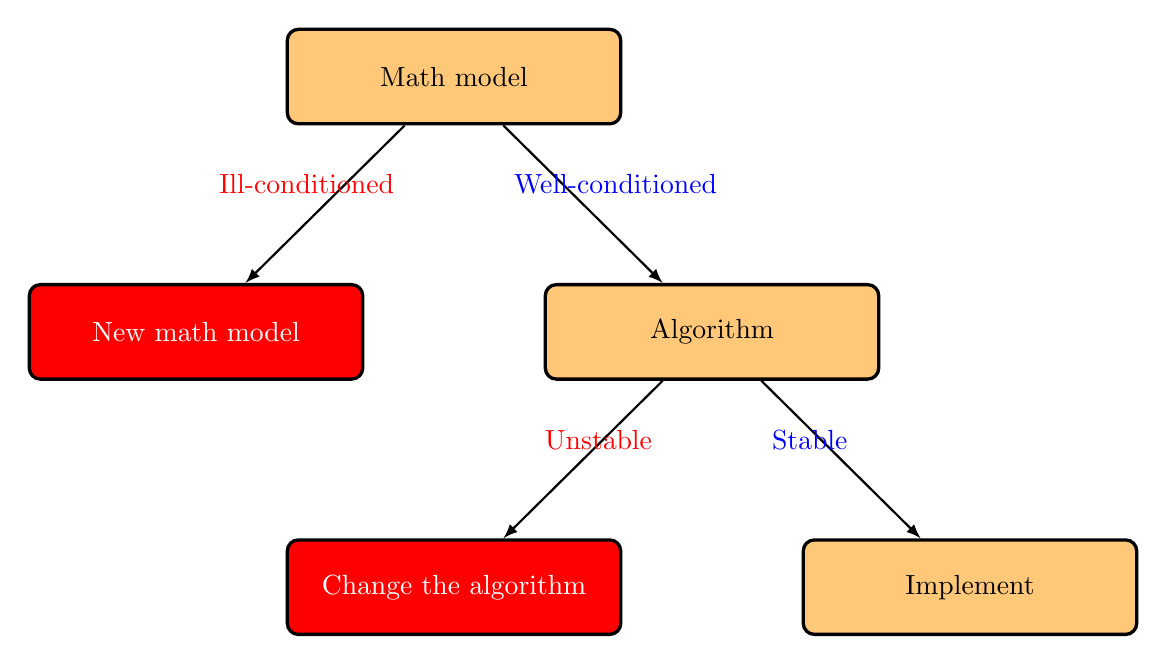
\begin{tikzpicture}
 	
 
 	\node [block] (m) {Math model} ;
 	\node [block, below right=2cm and -1cm of m] (a) {Algorithm};
    \node [blockr, below left=2cm and -1cm of m] (n) {\textcolor{white}{New math model}};
 	\node [blockr, below left=2cm and -1cm of a] (na) {\textcolor{white}{Change the algorithm}};
 	\node [block, below right=2cm and -1cm of a] (p) {Implement};
 
 
 	\draw [arrow] (m) -- (a);
 	\draw [arrow] (m) -- (n);
 	\draw [arrow] (a) -- (p);
 	\draw [arrow] (a) -- (na);
 	
 
 
 
 	
 
 	\node [color=blue, below right=0.5cm and -1.5cm of m ]  {Well-conditioned};
 	\node [color=red, below left=0.5cm and -1.5cm of m ]  {Ill-conditioned};
 	\node [color=blue, below right=0.5cm and -1.5cm of a ]  {Stable};
 	\node [color=red, below left=0.5cm and -1.5cm of a ]  {Unstable};
 
 
 	
 	
 	\end{tikzpicture}
 	
 	\caption{Software Development Life Cycle }
 \end{figure}





  

\newpage    
\section{Common numerical errors}

    
    
\listings{\home/Round_off.f90}
{errors_in_operations}{end subroutine}
{Round_off.f90} 



\newpage    
\section{Catastrophic cancellation}  \label{sec:cancellation}
    
    
\listings{\home/Round_off.f90}
{catastrophic_cancellation}{end subroutine}
{Round_off.f90} 





\newpage    
\section{Truncation errors and round-off errors}
    
     
\listings{\home/Summation_errors.f90}
{summation_example}{end subroutine}
{Summation_errors.f90} 



\newpage    
\section{IEEE exception examples}
    
    
\listings{\home/IEEE_operations.f90}
{IEEE_exception_examples}{end subroutine}
{IEEE_operations.f90} 






\section{TO MERGE}


1. Calculando el epsilon correcto suma hasta un cierto error en modo debug
2. En ese caso Debug sumar 10000000 de terminos no supone diferencia porque son numeros que no se pueden sumar ya
3. Sumar hacia atras si reduce enormemente el errror de floating en cada suma y consigue mucha mas exactitud

4.Pero la suma hacia delante si se hace con el modo Release optimiza el bucle y calcula con  mas precision 10000000 de terminos de la suma que el caso en el que para en el epsilon que le corresponde. Esto es magia del compilador que optimiza y seguramente haga sumas parciales hacia atras y por eso da mas exactitud. 

5. Correr en modo release pero pedir que lo pinte dentro del bucle hace lo mismo que debug porque no es capaz de aplicar la optimizacion si le pides que pinte cosas entre medias. 

In the context of floating-point representation, the intrinsic function $\epsilon$ represents the smallest 
number that added to 1 results in a number higher than 1.
This value depends on the number of binary digits reserved to store the floating-point
value (as it is covered in the section \ref{chap:reals}). 

It seems clear that adding a number higher than $\epsilon/2$ to 1
will be captured by the floating-point precision jumping to the value $1 + \epsilon$, a lower value will not be added
since the result is closer to 1 (and further from $1 + \epsilon$). For a number different than 1, let's say for example $S = 12.54$ a slight 
modification of the epsilon is needed. However, the idea is the same, the floating-point value does not allow 
adding more terms to $ S $ when those values are less than $\epsilon/2$. 


%Notice that $S(1 + \epsilon) = S + S\epsilon$ represents an upper bound 
%for the nearest floating-point value to $S$. Hence, adding values smaller than $S\epsilon$ to the number $S$ 
%will not be captured in the result. 




%First, take a look at the result of the computer if the summation process is stopped according to the 
%floating-point error due to the significant digits. Notice that this result is obtained after 2260 sums
%and the truncation error has the main part.
%
%\begin{verbatim} 
%    Total Error = 4.4035912E-04
%    Truncation Error = 4.4247787E-04
%    Floating-point Error = -2.1187589E-06
%\end{verbatim}
%
%Now try to calculate the same sum up to 10000000 terms, notice that the total error is similar to the 
%previous case, a little lower at cost of 4 thousand times the number of sums performed, 
%but now the floating-point error has the main contribution for the total error. 
%
%\begin{verbatim} 
%    Total Error = 2.0885468E-04
%    Truncation Error = 1.0000000E-07
%    Floating-point Error = 2.0875467E-04
%\end{verbatim}
%
%In addition, there is another way of calculating this sum with better accuracy in the computer apart from 
%using higher precision for the variables. This is a non-intuitive way of calculating the sum that comes from the fact
%that adding in floating-point arithmetic is not an associative operation. 
%Let's perform the same sum backwards, with simple precision also and from the lower terms to the higher ones using 10000000 terms. 
%
%\begin{verbatim} 
%    Total Error = 2.3841858E-07
%    Truncation Error = 1.0000000E-07
%    Floating-point Error = 1.3841859E-07
%\end{verbatim}
%
%As a general rule, when adding terms with really different orders of magnitude try to sum first the lower values and then add the result to the higher values.



%An extensive discussion regarding the consistency of using \texttt{epsilon( S )} for this example and the generalization for any other sum 
%is treated in the section \ref{chap:reals} of Part \ref{PartII} of this book. Also, why dividing it by \texttt{2} is needed becomes clearer. Some notions of 
%floating-point representation are essential to deepen in these topics. 
